\chapter{Experiments}
\label{cha:experiments}

\section{Experimental Setup}
\label{sec:experimental-setup}

\begin{comment}
Trying and failing is a major part of research. However, to have a chance of success you need a plan driving the experimental research, just as you need a plan for your literature search. Further, plans are made to be revised and this revision ensures that any further decisions made are in line with the work already completed.

The plan should include what experiments or series of experiments are planned and what questions the individual or set of experiments aim to answer. Such questions should be connected to your research questions, so that in the evaluation of your results you can discuss the results wrt to the research questions.
\end{comment}

\begin{comment}
The experimental setup should include all data --- parameters, etc. --- that would allow a person to repeat your experiments.
This will thus be the actual instantiation for each experiment of the general architecture described in Chapter~\ref{cha:architecture}.
\end{comment}

The experiments conducted to evaluate the performance of GeoGPT on geospatial tasks are divided into two approaches. The first approach, elaborated upon in \autoref{subsec:benchmarking-setup}, is intended to evaluate GeoGPT's ability to solve a variety of geospatial tasks. The second approach, presented in \autoref{subsec:prompt-quality-test-setup}, aims to uncover the importance of the initial user prompt in guiding GeoGPT to solve the task. \Autosubsectionref{subsec:configuration-and-hardware} describes the hardware on which the experiments were executed, and the specific models that were used.

\subsection[GIS Q\&A Experiment]{\acrshort{acr:gis} Q\&A Experiment}
\label{subsec:benchmarking-setup}

The first approach seeks to evaluate its ability to successfully answer questions that have a concrete answer. To do this, a Q\&A dataset was constructed. This dataset consists of set of 12 GIS-related questions with corresponding correct answers. For each record in the dataset, a description of how a human would find it natural to approach the problem. This description is provided as a step-by-step path towards the solution, and is only included to guide any reader as to how the system would be expected to solve the system. The full Q\&A dataset can be found in \autoref{tbl:questions-quantitative}. This set of experiments will allow for quantitative assessment of GeoGPT's GIS-abilities, and is a feasible way of benchmarking the system.

Another aspect that the benchmarking approach will try to evaluate is the consistency of the system, its ability to repeatedly provide an acceptable answer to the same user question. Each of the 12 questions are therefore asked three times per agent type.

With the implementation of three different agent types, the total number of test runs becomes the following: $$12 \text{ questions} \cdot 3 \text{ agent types} \cdot 3 \text{ repetitions} = 108 \text{ tests}$$


\subsubsection{Outcome Evaluation}

Each test run's answer will be manually evaluated, and the outcome will be annotated as one of \textit{success}, \textit{partial success}, and \textit{failure}. \autoref{tbl:test-outcome-enum} shows the guidelines used when assigning test results.

\begin{table}[htbp]
    \centering
    \caption{Description of Success}
    \label{tbl:test-outcome-enum}
    \begin{tabularx}{0.9\textwidth}{p{3cm}X}
        \toprule
        \textbf{Outcome} & \textbf{Guideline}                                                                                                                                                                                  \\
        \midrule
        Success          & The question was answered correctly and little to no follow-up from the user was required to produce the desired outcome. No false assumptions were made by the system when answering the question. \\
        Partial Success  & Portions of the question were answered correctly or semi-correctly, and/or some follow-up from the user was required to guide the system toward the solution.                                       \\
        Failure          & The question was answered incorrectly answered and/or false assumptions were made by the system while attempting to answer the question.                                                            \\
        \bottomrule
    \end{tabularx}
\end{table}

The annotated outcomes are then encoded using the ordinal encoding presented \autoref{tbl:outcome-encoding}. A higher value indicates a better outcome. These encoded outcome values enable standard deviation calculations, which serve as a suitable measure for assessing repeatability. This approach also allows for comparisons across different agent types and configurations.

\begin{table}[htbp]
    \centering
    \caption{Encoding for Test Outcome}
    \label{tbl:outcome-encoding}
    \begin{tabularx}{0.5\textwidth}{XX}
        \toprule
        \textbf{Outcome} & \textbf{Encoded Value} \\
        \midrule
        Success          & 2                      \\
        Partial Success  & 1                      \\
        Failure          & 0                      \\
        \bottomrule
    \end{tabularx}
\end{table}


\subsubsection{Cost and Duration}

The application is hooked up to LangChain AI's tracing system, \textit{LangSmith}. Apart from being a useful tool for debugging purposes, it provides a simple way of obtaining detailed data for token and time usage for a particular run, as well as the total cost of the run. These are metrics that will be recorded and used in the evaluation of GeoGPT.

To summarize, the following metrics are recorded for a given test run:

\begin{itemize}
    \item The outcome of the test (\textit{success}, \textit{partial success}, or \textit{failure})
    \item The total duration in seconds
    \item The total number of tokens used
    \item The total cost for the run in American dollar
\end{itemize}


\subsection{Prompt Quality Experiment}
\label{subsec:prompt-quality-test-setup}

The second set of experiments are constructed to evaluate the importance of the initial question/prompt from the human user. As stated in \nameref{sec:background-and-motivation}, part of the motivation for developing an \acrshort{acr:llm}-driven \acrshort{acr:gis} like GeoGPT is to make \acrshort{acr:gis} more accessible to non-experts. At the same time, it may be valuable to assess the extent to which a carefully constructed prompt by a GIS expert can enhance the system's output.


\subsection{Configuration and Hardware}
\label{subsec:configuration-and-hardware}

All experiments were executed locally on a Lenovo ThinkPad E490, which has an Intel{\textregistered} Core\texttrademark{} i7-8565U CPU @ 1.80GHz processor, 15.8 GB usable \acrshort{acr:ram}, and 256 GB \acrshort{acr:ssd} storage. Everything but the \acrshort{acr:llm} inference was executed locally. Text generation was done using OpenAI's \acrshort{acr:api}.

It is worth noting that two slightly different models were used during testing. The explanation of this is the release of the \texttt{gpt-4-turbo-2024-04-09} in mid-April. According to OpenAI, \enquote{this new model is better at math, logical reasoning, and coding} compared to \texttt{gpt-4-0125-preview}\footnote{OpenAI has a GitHub repository containing the code they use to evaluate their \glspl{acr:llm} and benchmark results for OpenAI models and reference models from other companies: \url{https://github.com/openai/simple-evals}.}, which is the model that was used at the start of the experimentation phase of the master's thesis. At the new model's release, a decision was made to use this for the remaining experiments. The experiments that had already been conducted were not re-run due to time constraints and a belief that these slight model upgrades would not significantly change the outcome of the experiments.


\section{Experimental Results}
\label{sec:experimental-results}

\begin{comment}
Results should be clearly displayed and should provide a suitable representation of your results for the points you wish to make.
Graphs should be labelled in a legible font. If more than one result is displayed in the same graph, then these should be clearly marked.
Please choose carefully rather than presenting every result. Too much information is hard to read and often hides the key information you wish to present. Make use of statistical methods when presenting results, where possible to strengthen the results.
Further, the format of the presentation of results should be chosen based on what issues in the results you wish to highlight.
You may wish to present a subset in the experimental section and provide additional results in an appendix.
Point out specifics here but save the overall/general discussion to the Discussion chapter.
\end{comment}

\Autosubsectionref{subsec:quantitative-results} and \autoref{subsec:prompt-quality-test-results} will present the outcome of the experiments presented in \autoref{subsec:prompt-quality-test-setup} and \autoref{subsec:prompt-quality-test-setup}, respectively.


\subsection[GIS Q\&A Experiment --- Results]{\acrshort{acr:gis} Q\&A Experiment --- Results}
\label{subsec:quantitative-results}

Graphs created for this chapter are created using Matplotlib\footnote{\url{https://matplotlib.org/}}, a Python library suitable for creating visualizations like bar charts, box plots, etc.

\subsubsection{Outcomes}

As described in \autoref{subsec:benchmarking-setup}, a total 108 tests were run using the 12 available Q\&A samples, with the same question being repeated three times for each of the three agent types \todo{ref some table with agent types}, resulting in 36 test runs per agent. \autoref{fig:outcome-distribution} displays a bar chart for the outcome distribution per agent.


\begin{figure}[htbp]
    \centering
    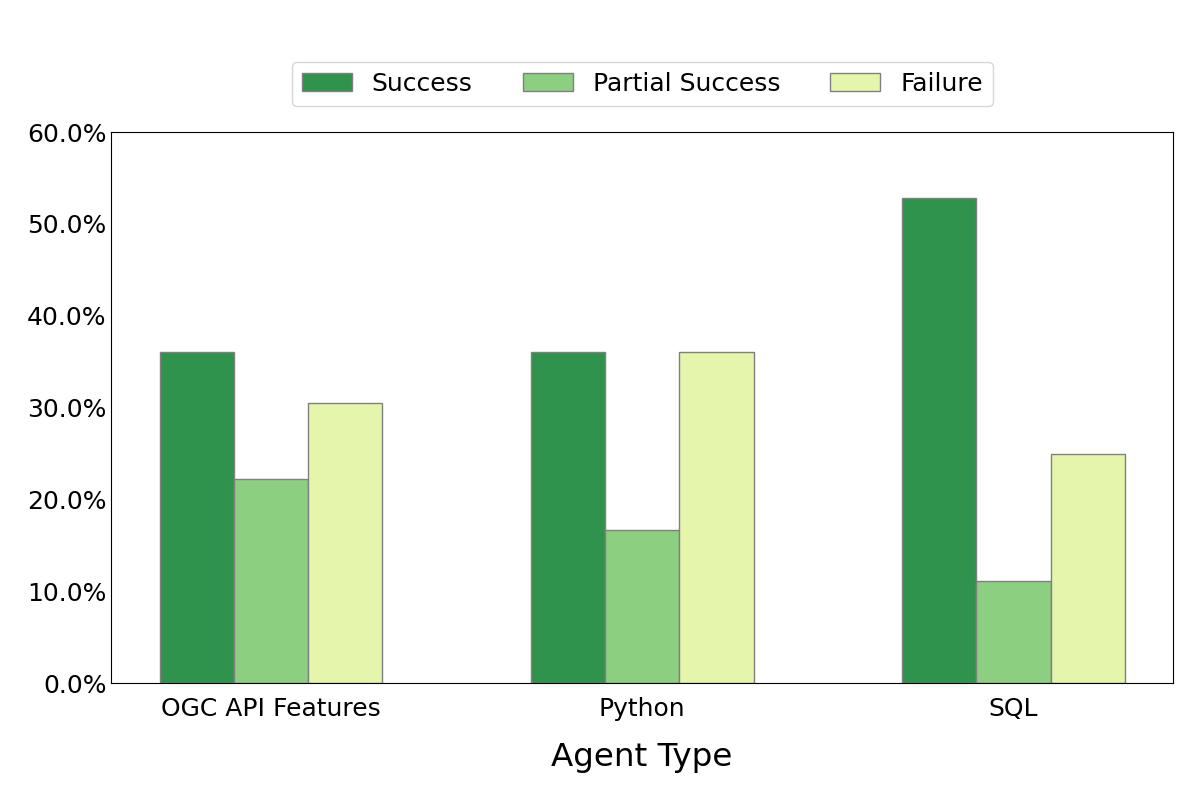
\includegraphics[width=\textwidth]{outcome_distribution_bar_chart.png}
    \caption{Outcome distribution between different agent types}
    \label{fig:outcome-distribution}
\end{figure}

From \autoref{fig:outcome-distribution}, we can read that the \acrshort{acr:ogc} \acrshort{acr:api} Features and Python agent have comparable results, and that the \acrshort{acr:sql}-based agent performs significantly better compared to the other two in terms of producing the desired outcome.

\subsubsection{Cost and Duration}

This section features three different box plots: \autoref{fig:duration-box-plot}, \autoref{fig:cost-box-plot}, and \autoref{fig:tokens-box-plot}. The Matplotlib implementation of the box plot follows the description found on Wikipedia\footnote{\url{https://matplotlib.org/stable/api/_as_gen/matplotlib.pyplot.boxplot.html}}\footnote{\url{https://en.wikipedia.org/wiki/Box_plot}}. Box plots allow us to easily visualize where the 0th ($Q_0$), 25th ($Q_1$), 50th ($Q_2$), 75th ($Q_3$), and 100th ($Q_4$) percentiles of the datasets lie, as well as the dataset's outliers. Outliers are those data points fall outside 1.5 times interquartile range, that is, the distance between $Q_3$ and $Q_1$ in each direction.

\autoref{fig:duration-box-plot} displays a box plot with a logarithmic y-axis showing the relative durations for task completion across the different agent types. Here we can see that the \acrshort{acr:sql} agent spends the least amount of time per task, and that the \acrshort{acr:ogc} \acrshort{acr:api} Features agent has a slightly higher median but with a few time-consuming outliers. The Python agent is the odd one out with a median of $\sim 82$ seconds, a $Q3 \sim 293$ seconds, and a $Q4 \sim 984$. The large gap to the other two agents it largely due to the Python agent's tendency to load large datasets into memory without filtering the data on load using a bounding box. For instance, when attempting the task of calculating the difference between the polygon outlining Oslo and water polygons, the Python agent used nearly 40 minutes on the entire task. $94\%$ of the time was spent executing the code presented in \autoref{code:python-oslo-water-diff}. The main reason for the long execution time is line 8, where the whole \texttt{osm\_landuse\_polygons.shp} dataset is loaded into memory. This dataset has a size of 1,383 MB, and loading such amounts of data in this way is very time-consuming. The Python agent was the only agent with such issues because the \acrshort{acr:ogc} \acrshort{acr:api} Features agent is limited to 10,000 features per dataset and the \acrshort{acr:sql} agent does not load the data into memory like the other agents do.

\begin{figure}[htbp]
    \centering
    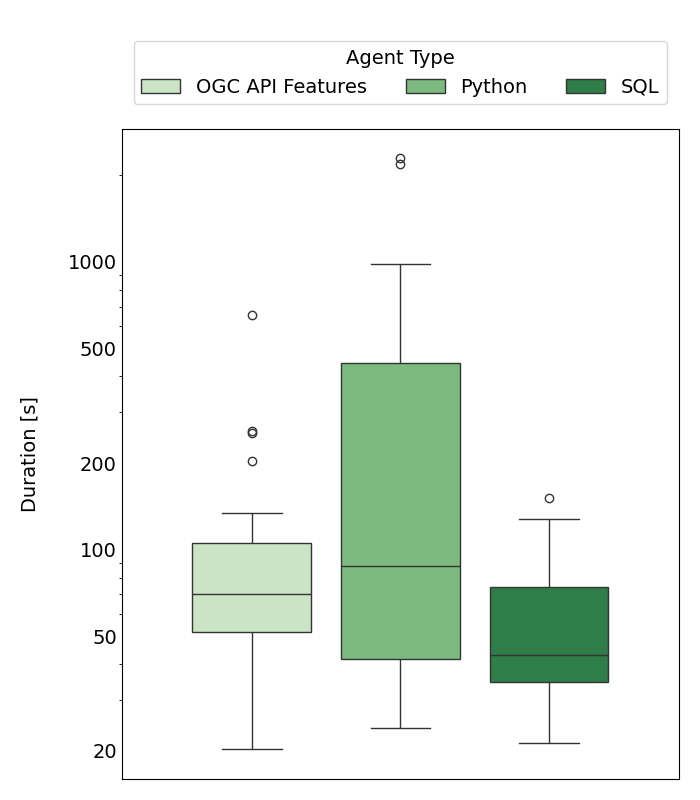
\includegraphics[width=0.6\textwidth]{duration_box_plot.png}
    \caption{Duration per Agent Type}
    \label{fig:duration-box-plot}
\end{figure}

\begin{lstlisting}[
    language=Python,
    caption=GeoGPT-generated Python code aimed at computing the difference between the Oslo outline and water features within it,
    label=code:python-oslo-water-diff,
    float, floatplacement=H
]
    import geopandas as gpd

    # Paths to the shapefiles
    landuse_path = '/tmp/tmpsutdy6it/osm_landuse_polygons.shp'
    places_path = '/tmp/tmpsutdy6it/osm_places_polygons.shp'
    
    # Load the data from shapefiles
    landuse_gdf = gpd.read_file(landuse_path)
    places_gdf = gpd.read_file(places_path)
    
    # Filter out 'residential' areas from the landuse data
    residential_gdf = landuse_gdf[landuse_gdf['fclass'] == 'residential']
     
    # Compute the spatial difference to exclude residential areas from the places data
    oslo_outline = gpd.overlay(places_gdf, residential_gdf, how='difference')
    
    # Path for the output GeoJSON file
    output_path = '/tmp/tmpsutdy6it/oslo_outline_no_residential.geojson'
    
    # Save the resulting GeoDataFrame to a GeoJSON file
    oslo_outline.to_file(output_path, driver='GeoJSON')
    
    # Output the path to the saved file
    print(output_path)    
\end{lstlisting}

\autoref{fig:cost-and-tokens} shows box plots for the amount of tokens used per run and the total cost of these. Naturally, these figures appear very similar, as OpenAI sets fixed prices for the input tokens and generated output tokens for their \acrshort{acr:gpt} models. According to their websites\footnote{\url{https://openai.com/pricing}}, they charge $\$10$ per million input tokens and $\$30$ per million output tokens for their \acrshort{acr:gpt}-4 Turbo models. From the results of the experiments, a ratio of approximately $10.7$ per million tokens --- either input \textit{or} output --- was calculated, which is very close to the input token price. This aligns with the observation that the number of input/prompt tokens is significantly greater than the number of output/generated tokens for the experiments conducted. The correlation matrix in \autoref{fig:correlation-matrix} confirms that this ratio is consistent.

\begin{figure}[htbp]
    \centering
    \begin{subfigure}[b]{0.48\textwidth}
        \centering
        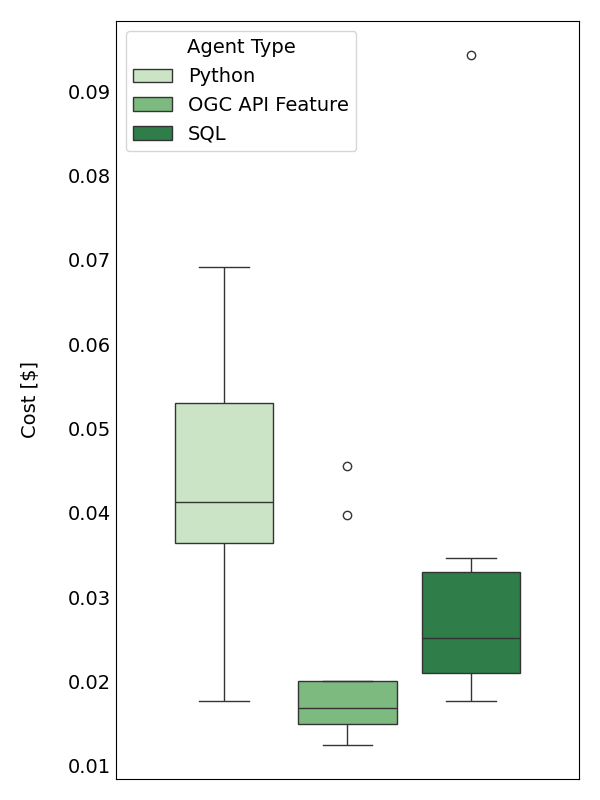
\includegraphics[width=\textwidth]{cost_box_plot.png}
        \caption{Average cost per call for each agent type}
        \label{fig:cost-box-plot}
    \end{subfigure}
    \hfill
    \begin{subfigure}[b]{0.48\textwidth}
        \centering
        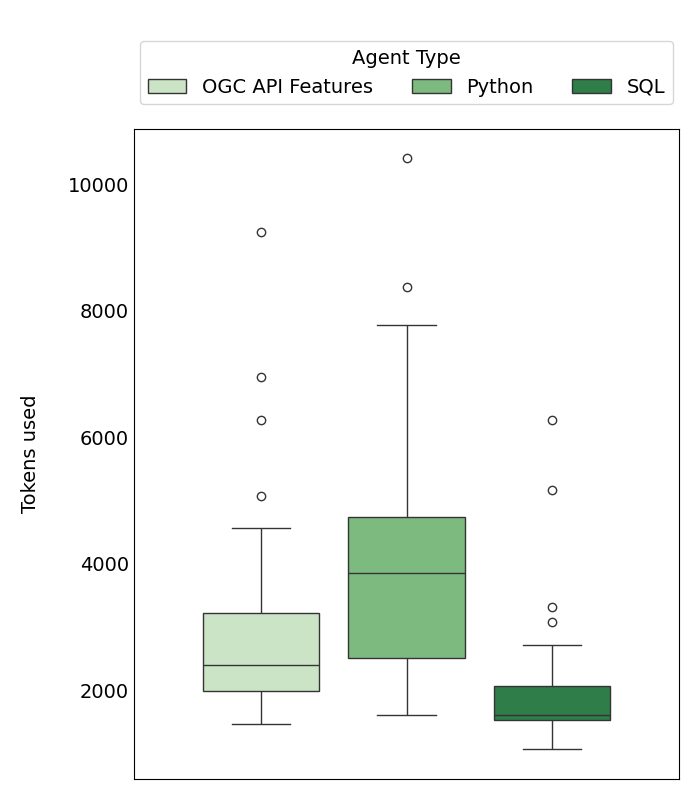
\includegraphics[width=\textwidth]{tokens_box_plot.png}
        \caption{Average token usage per agent type}
        \label{fig:tokens-box-plot}
    \end{subfigure}
    \caption{Cost and token usage}
    \label{fig:cost-and-tokens}
\end{figure}

Another observation that can be made from \autoref{fig:correlation-matrix} is that there is only a \textit{slight} positive correlation between duration and token/usage. This supports the observation that code execution time is likely the most significant factor in determining the duration required to complete a task for the datasets and tasks used in this thesis' experiments.

A third observation that can be made from the \autoref{fig:correlation-matrix} is the negative correlation between the encoded outcome and token usage, duration, and total cost. This suggests that A task that takes longer to complete --- and thus is likely to be more expensive in terms of token usage --- is more likely to produce an undesirable outcome. Possible reasons as to why this is the case will be explored in the \nameref{cha:discussion}.

\begin{figure}[htbp]
    \centering
    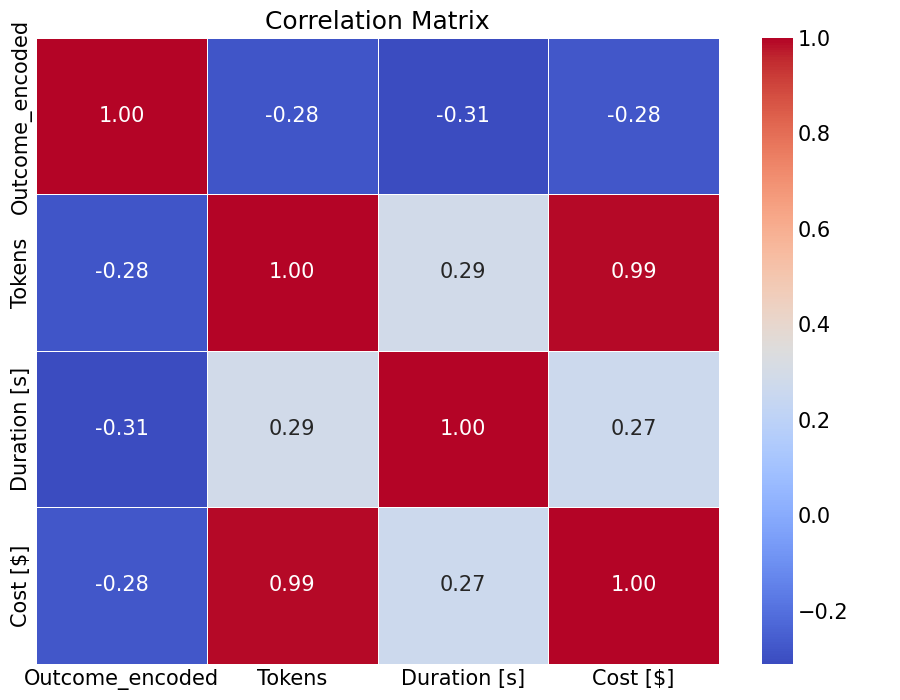
\includegraphics[width=0.7\textwidth]{correlation_matrix.png}
    \caption{Correlation matrix for test result metrics}
    \label{fig:correlation-matrix}
\end{figure}

\subsubsection{Repeatability}

\autoref{tbl:stddev-by-agent-type} shows the average standard deviation for each agent type, as well as the mean of these three standard deviations. The latter serves as an overall measure of GeoGPT's ability to repeatedly produce the desired outcome from a given query. Standard deviations were calculated for each triplet of identical test samples, in which both the question and the agent type remained the same. To produce a numerical value for the standard deviations, the encoded outcomes (see \autoref{tbl:outcome-encoding}) were used. Taking the average of the standard deviations for all 12 triplets for each agent type produced the numbers found in \autoref{tbl:stddev-by-agent-type}.These numbers indicate that there is a notable amount of inconsistency in GeoGPT's ability to produce correct answers, on an average deviating with almost \enquote{half an outcome category} (0.408 for the encoded values) for the same task and agent type.

\begin{table}[htbp]
    \centering
    \caption{Standard Deviation by Agent Type}
    \label{tbl:stddev-by-agent-type}
    \begin{tabularx}{0.7\textwidth}{XX}
        \toprule
        \textbf{Agent Type}                            & \textbf{Outcome Std. Deviation} \\
        \midrule
        \acrshort{acr:ogc} \acrshort{acr:api} Features & 0.552                           \\
        Python                                         & 0.337                           \\
        \acrshort{acr:sql}                             & 0.241                           \\
        \midrule
        \textbf{Mean}                                  & 0.376                           \\
        \bottomrule
    \end{tabularx}
\end{table}

\subsubsection{Successful Responses}

% 6df94421-6c7c-470a-af8e-7013f3bc547f
\autoref{fig:glomma-counties-sql-successful} shows a successful response from GeoGPT's \acrshort{acr:sql} agent when asked how many counties the Glomma river runs through.\footnote{This run was not part of the results used for evaluation due to a bug in the \acrshort{acr:sql} agent that caused the \texttt{sql\_db\_query} to unnecessarily execute many queries twice. GeoGPT's response would not be different had the bug not been present for the run, but it would have taken a bit longer to complete.} As a final answer to the initial prompt it lists all four correct counties in a numbered list. \autoref{code:glomma-counties-sql} shows the code generated by GeoGPT for the second invocation of \texttt{sql\_db\_query}. The second invocation is nearly identical to the first one, but in the first invocation the geometry column --- named \enquote{geom} --- was not included in the response, something the tool informs GeoGPT of in its tool message. GeoGPT therefore decided to run the query again, now making sure to include the geometry column in the query result, before adding the result to the map using \texttt{add\_geojson\_to\_map}. A follow-up message instructed GeoGPT to \enquote{Add Glomma to the map}, allowing for visual verification that the results were correct.

\begin{figure}[h]
    \centering
    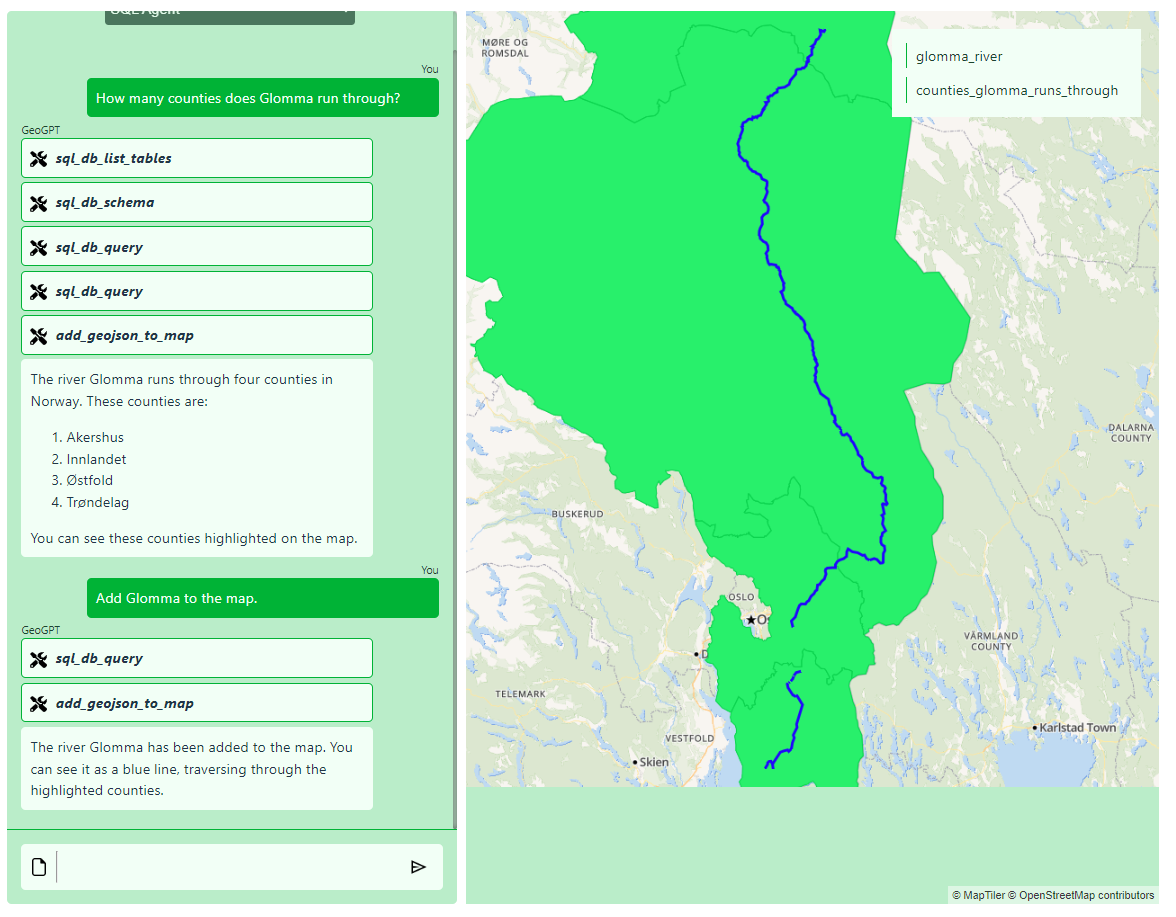
\includegraphics[width=0.7\textwidth]{glomma_counties_sql_22.png}
    \caption{Successful response from GeoGPT's \acrshort{acr:sql} agent when asked how many counties the Glomma river runs through}
    \label{fig:glomma-counties-sql-successful}
\end{figure}

\begin{lstlisting}[
    language=sql,
    caption=SQL code generated by GeoGPT to retrieve polygons of the counties that the Glomma river runs through,
    label=code:glomma-counties-sql
]
WITH river AS (
    SELECT geom 
    FROM osm_waterways_lines 
    WHERE fclass = 'river' AND name ILIKE 'Glomma'
),

places AS (
    SELECT geom, name 
    FROM osm_places_polygons 
    WHERE fclass = 'county'
)

SELECT DISTINCT places.name AS county_name, places.geom AS geom
FROM river, places
WHERE ST_Intersects(river.geom, places.geom);    
\end{lstlisting}

\autoref{fig:trees-along-munkegata-python-partial-success} shows a partially successful attempt from GeoGPT's Python agent to calculate the number of trees along Munkegata in Trondheim. While setting a definitive answer is difficult, the correct answer was set to about 100 trees when using a buffer of 20 meters around the line segments that make up the road.

\begin{figure}[h]
    \centering
    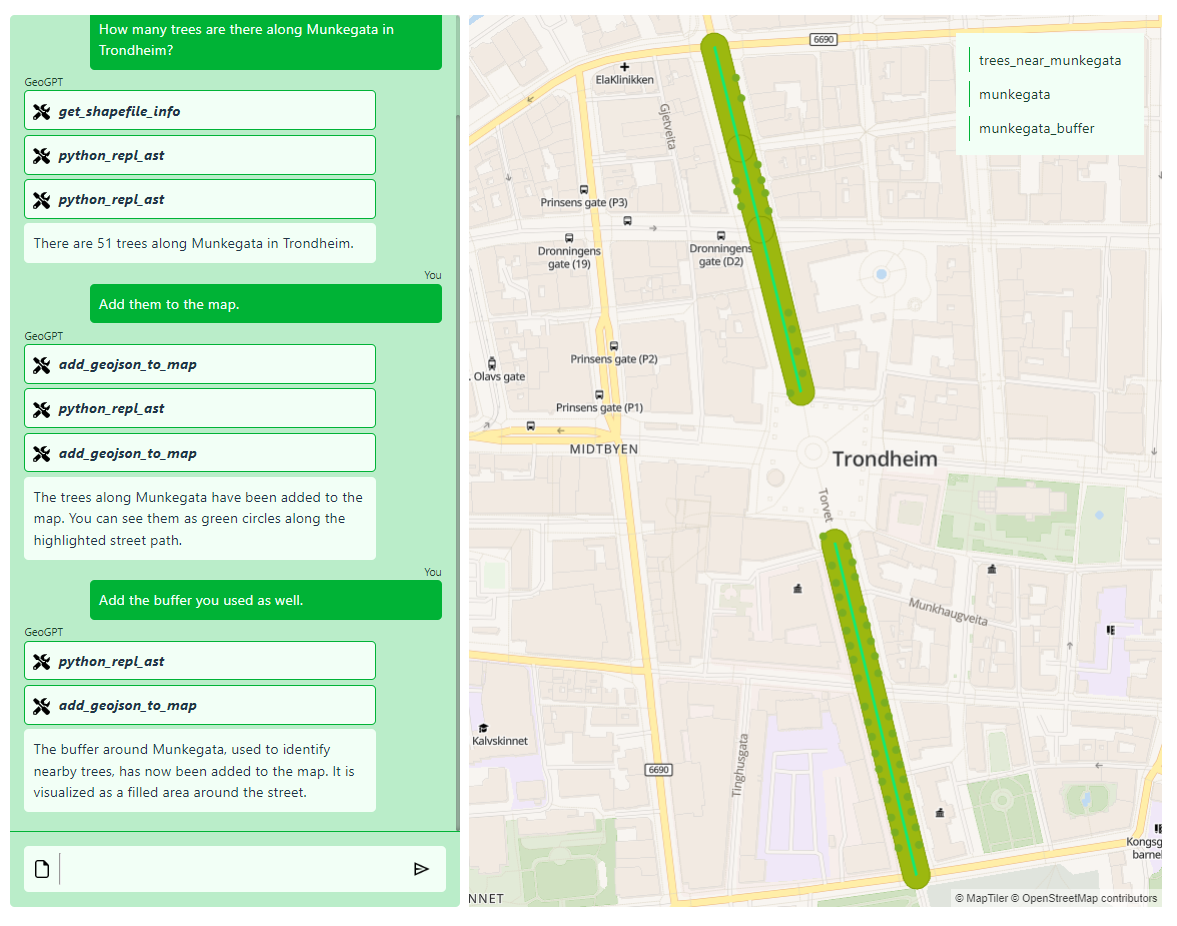
\includegraphics[width=0.7\textwidth]{num_trees_along_munkegata_python_with_buffer.png}
    \caption{Partially successful response from GeoGPT's Python agent when asked how many trees there are along Munkegata in Trondheim}
    \label{fig:trees-along-munkegata-python-partial-success}
\end{figure}

\begin{lstlisting}[
    language=python,
    caption=Python code to exclude roads named Munkegata \textit{outside} of Trondheim,
    label=code:python-munkegata-bbox
]
import geopandas as gpd

# Load roads data with a focus on Munkegata
roads_path = '/tmp/tmpl8zsdj6m/osm_roads_lines.shp'
munkegata_bbox = (10.3910, 63.4270, 10.4030, 63.4330) # Approximate bounding box around Munkegata
munkegata_roads = gpd.read_file(roads_path, bbox=munkegata_bbox)

# Filter for Munkegata
munkegata = munkegata_roads[munkegata_roads['name'] == 'Munkegata']

# Save filtered Munkegata road to GeoJSON
munkegata_path = '/tmp/tmpl8zsdj6m/munkegata.geojson'
munkegata.to_file(munkegata_path, driver='GeoJSON')

print(munkegata_path)
\end{lstlisting}

\begin{lstlisting}[
    language=python,
    caption=Python code to calculate the number of trees along Munkegata in Trondheim,
    label=code:python-trees-count-munkegata
]
from shapely.geometry import box
import geopandas as gpd

# Load the trees points
natural_points_path = '/tmp/tmpl8zsdj6m/osm_natural_points.shp'
trees = gpd.read_file(natural_points_path)

# Filter for trees
trees = trees[trees['fclass'] == 'tree']

# Load Munkegata road
munkegata_path = '/tmp/tmpl8zsdj6m/munkegata.geojson'
munkegata_road = gpd.read_file(munkegata_path)

# Project to UTM for accurate distance measurement
munkegata_utm = munkegata_road.to_crs(epsg=32633)
trees_utm = trees.to_crs(epsg=32633)

# Buffer Munkegata by 10 meters to include nearby trees
tree_buffer = munkegata_utm.buffer(10)

# Spatial join trees within buffered Munkegata
trees_near_munkegata = gpd.sjoin(trees_utm, gpd.GeoDataFrame(geometry=tree_buffer), how='inner', op='intersects')

# Count the number of trees
tree_count = trees_near_munkegata.shape[0]
print(tree_count)

\end{lstlisting}

\subsubsection{Unsuccessful Responses}

While GeoGPT was able to get a lot of questions correct, it provided more or less unsuccessful answers at least once for all questions but one.

\autoref{fig:python-high-speed-roads-unsuccessful} exemplifies a common mistake with GeoGPT's agents which is a central topic in the \nameref{cha:discussion}. Here, the Python agent has failed to recognise that the road datasets it has available is in fact for the whole of Norway. As \autoref{code:python-high-speed-unsuccessful} shows, the agent performs the correct analysis based on the assumptions it has already made, but the answer is far from what the user enquired.

\begin{figure}
    \centering
    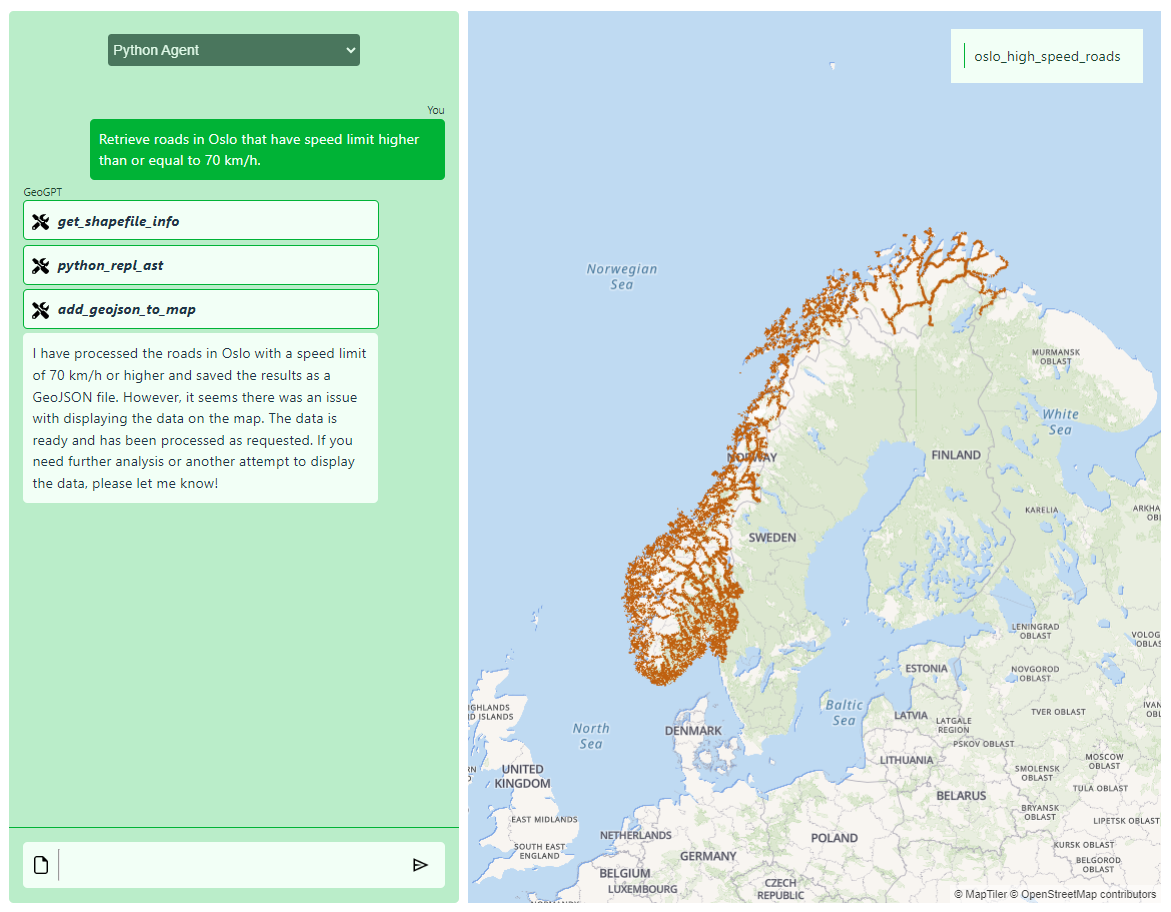
\includegraphics[width=0.7\textwidth]{oslo_roads_maxspeed_hte_70_kmh_python.png}
    \caption{Unsuccessful attempt by GeoGPT's Python agent to retrieve high-speed roads in Oslo}
    \label{fig:python-high-speed-roads-unsuccessful}
\end{figure}

\begin{lstlisting}[
    language=python,
    caption=Python code that saves high-speed roads with a misleading filename,
    label=code:python-high-speed-unsuccessful
]
import geopandas as gpd

# Define the file path for the roads shapefile
shapefile_path = '/tmp/tmpr1hvr_c5/osm_roads_lines.shp'

# Read the shapefile with a condition on maxspeed being >= 70
roads_gdf = gpd.read_file(shapefile_path)
roads_high_speed_gdf = roads_gdf[roads_gdf['maxspeed'].astype(float) >= 70]

# Save the filtered GeoDataFrame as GeoJSON
output_geojson_path = '/tmp/tmpr1hvr_c5/oslo_high_speed_roads.geojson'
roads_high_speed_gdf.to_file(output_geojson_path, driver='GeoJSON')

print(output_geojson_path)
   
\end{lstlisting}

\begin{figure}
    \centering
    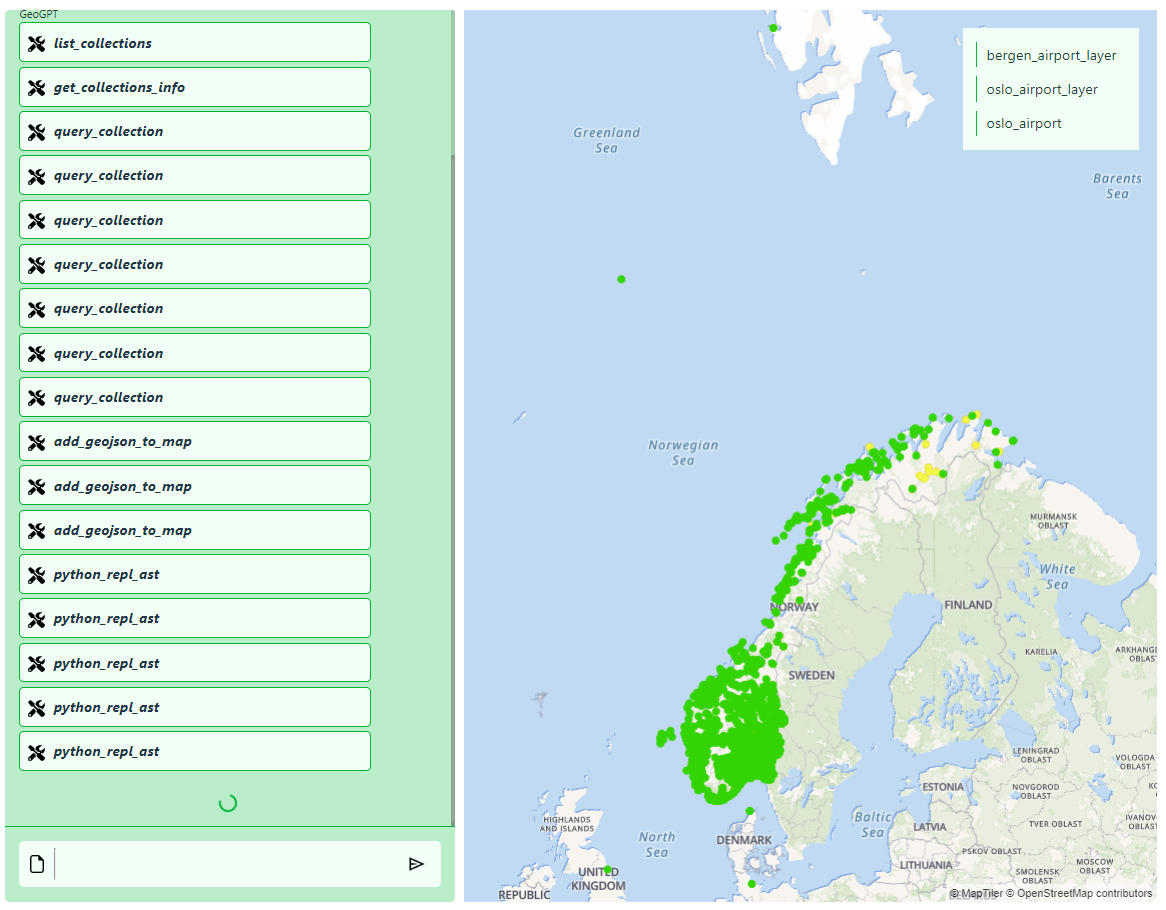
\includegraphics[width=0.7\textwidth]{oslo_bergen_geodesic_oaf2.png}
    \caption{Unsuccessful attempt by GeoGPT's \acrshort{acr:ogc} \acrshort{acr:api} Features agent to create a geodesic line between Oslo Airport Gardermoen and Bergen Airport Flesland}
    \label{fig:oaf-geodesic-unsuccessful}
\end{figure}

\subsection{Prompt Quality Experiment --- Results}
\label{subsec:prompt-quality-test-results}

\begin{figure}[htbp]
    \centering
    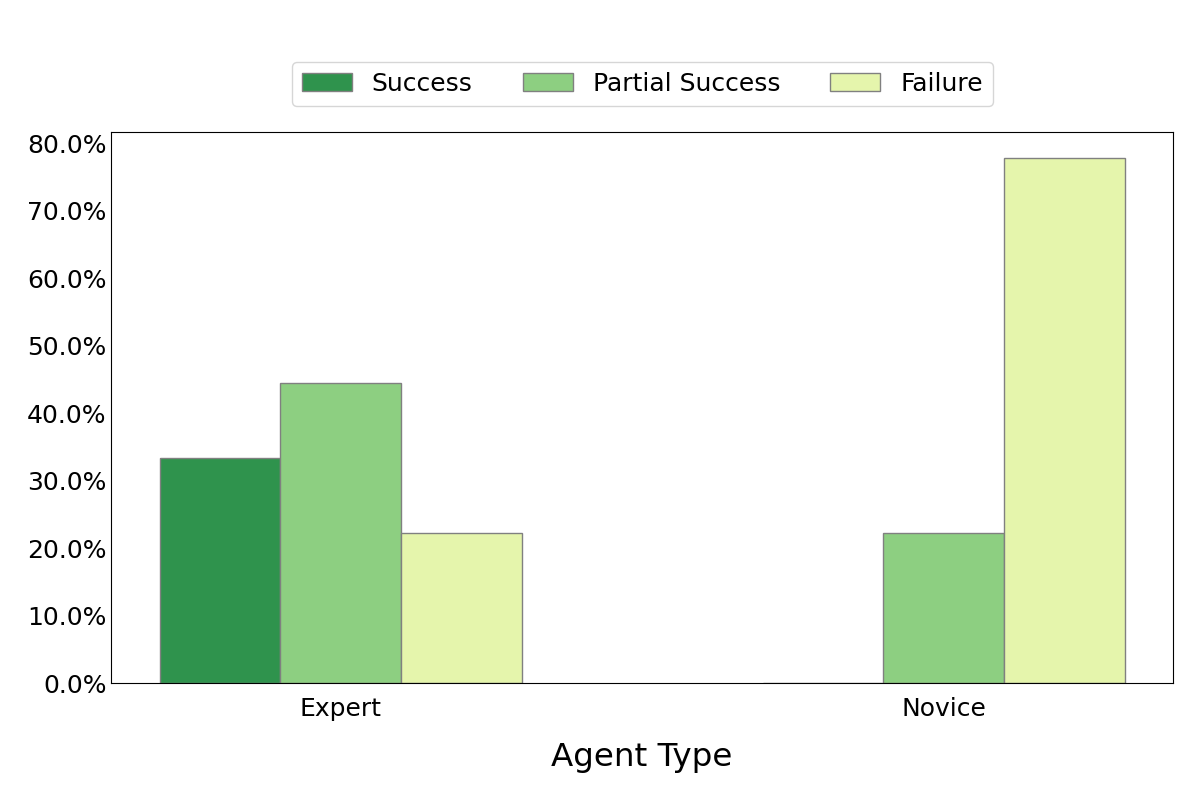
\includegraphics[width=\textwidth]{levels_outcome_distribution_bar_chart.png}
    \caption{Outcome distribution for different levels of GIS experience}
    \label{fig:outcome-distribution-experience-levels}
\end{figure}

\autoref{fig:novice-vs-expert-munkegata-trees} shows a comparison between the results GeoGPT managed to produce for two different prompts that one would expect to produce identical outcomes. The \textit{novice}-level prompt was as follows:

\begin{quote}
    \enquote{Could you count how many trees there are on Munkegata street in Trondheim?}
\end{quote}

\noindent The \textit{expert}-level prompt, on the other hand, included a series of instructions:

\begin{quote}
    \enquote{1. List all datasets that could possibly include trees. \\
        2. Find the correct feature class and filter the relevant dataset to access tree data for Trondheim. Use a bounding box to reduce the number of trees to analyse. \\
        4. Fetch road data for Munkegata. Use a bounding box for Trondheim in case there are streets elsewhere named Munkegata. \\
        5. Convert both datasets to a suitable metric CRS and add a 20-meter buffer around the road data. \\
        6. Find all trees that lie within this buffer and count them. \\
        7. Present the findings with a map highlighting the roads and the trees.}
\end{quote}

Using novice-level prompt GeoGPT was unable to produce the correct outcome, and confidently answered that there are \enquote{approximately 6,915 trees on Munkegata street in Trondheim.} (see \autoref{fig:novice-level-prompting-munkegata-trees}), which is far from being true. When solving the task, GeoGPT made a series of oversights that lead to this result. First, GeoGPT failed to take into account that there may be more than one street in the dataset with the name \enquote{Munkegata}, \enquote{forgetting} to use a bounding box when retrieving the road data from the \acrshort{acr:api}. The same mistake was made when retrieving the tree data. Due to the upper limit of 10,000 features per query in the \acrshort{acr:api}, it's crucial to narrow down the query to ensure retrieval of all relevant features rather than just a subset. GeoGPT's query for tree data lacked a bounding box, resulting in a randomly distributed subset scattered across Norway. A third mistake occurred when GeoGPT calculated a bounding box around the retrieved road data instead of creating a buffer. The latter method would have produced a more accurate result. The bounding box that was created spanned from Trondheim to Oslo, thus including far more trees than was intended.

On the other hand, the expert-level prompt provided the necessary guidance for GeoGPT for this specific task, steering it clear of the issues it encountered with the novice-level prompt. As stated by OpenAI themselves, \enquote{some tasks are best specified as a sequence of steps}.\footnote{\url{https://platform.openai.com/docs/guides/prompt-engineering/strategy-write-clear-instructions}} Furthermore, they say that writing explicit steps required to solve a tasks \enquote{makes it easier for the model to follow them}.

\begin{figure}[htbp]
    \centering
    \begin{subfigure}[b]{0.7\textwidth}
        \centering
        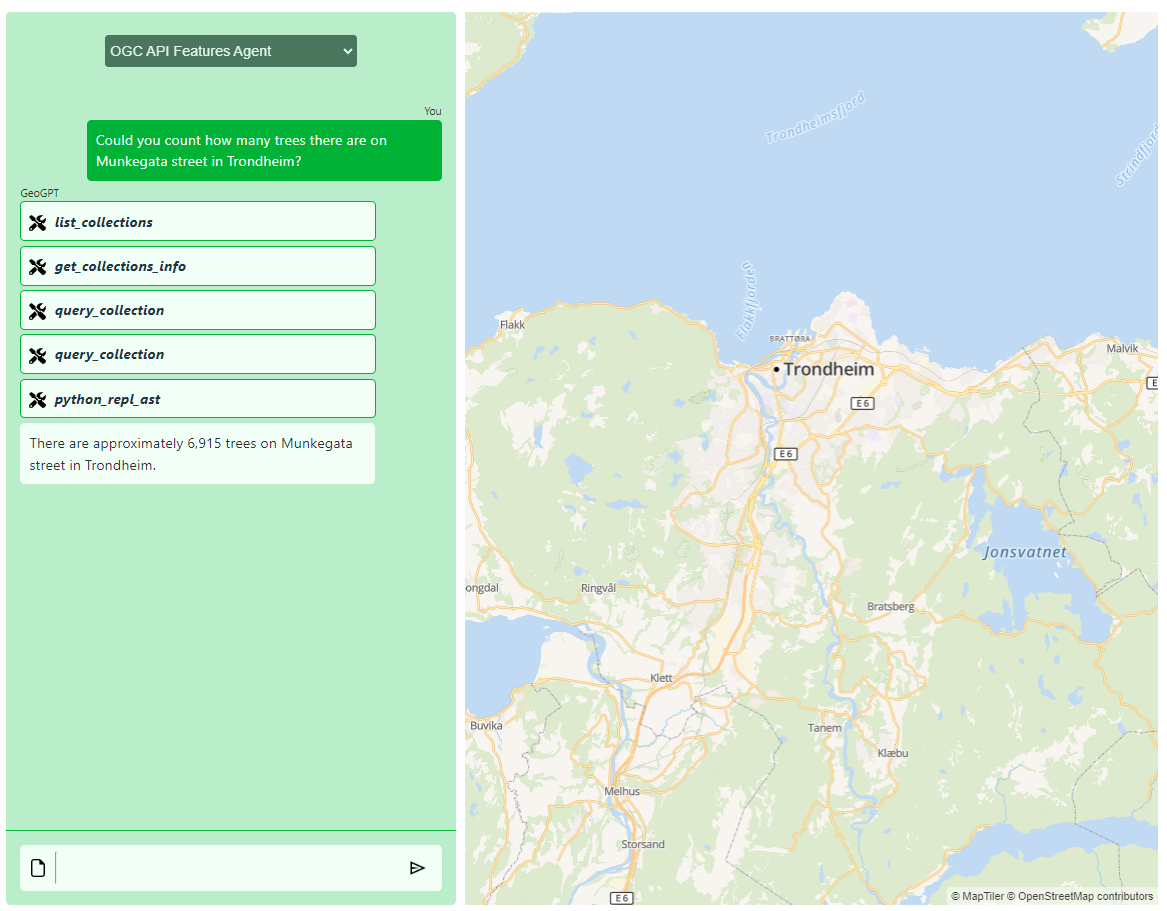
\includegraphics[width=\textwidth]{munkegata_trees_oaf_novice.png}
        \caption{Novice-level prompting}
        \label{fig:novice-level-prompting-munkegata-trees}
    \end{subfigure}
    \hfill
    \begin{subfigure}[b]{0.7\textwidth}
        \centering
        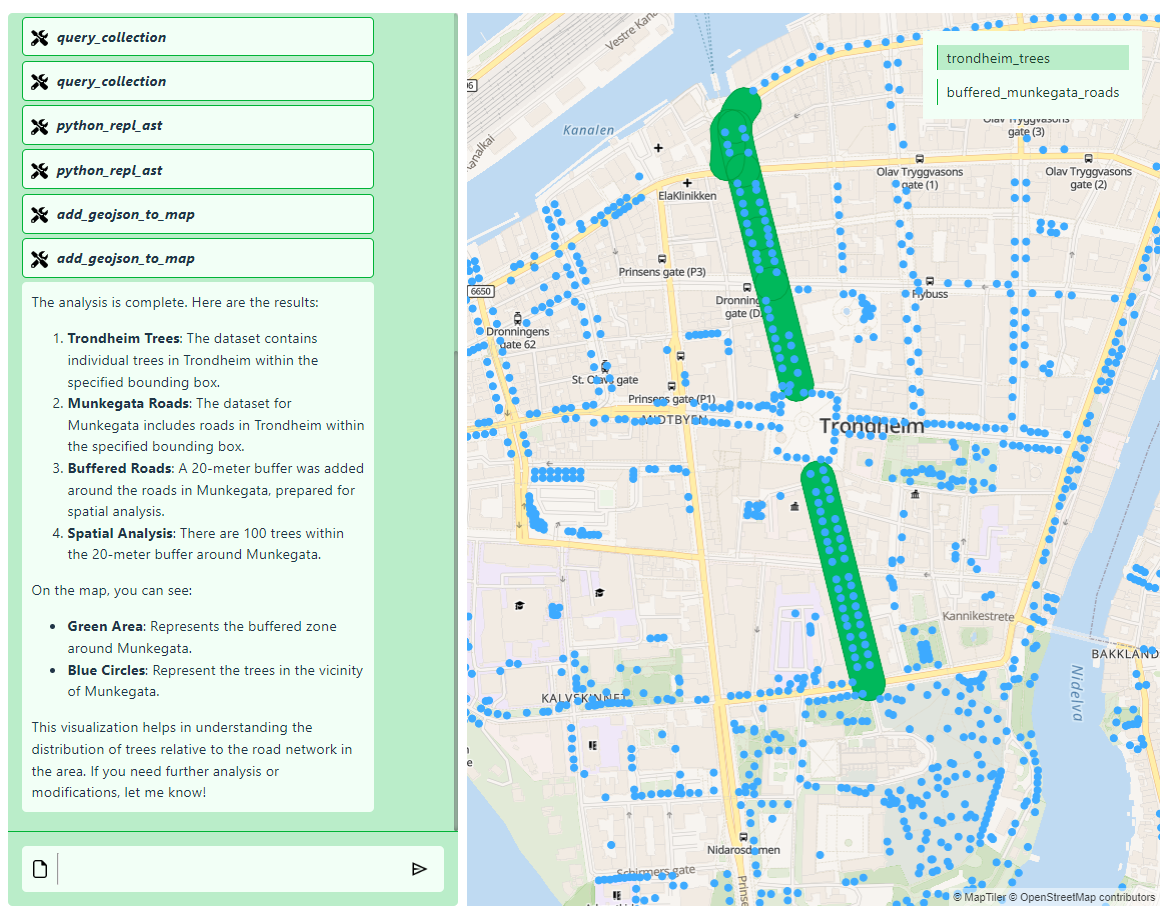
\includegraphics[width=\textwidth]{munkegata_trees_oaf_expert_sbs_2.png}
        \caption{Expert-level prompting}
        \label{fig:expert-level-prompting-munkegata-trees}
    \end{subfigure}
    \caption{Comparison between novice- and expert-level prompting of GeoGPT's \acrshort{acr:ogc} \acrshort{acr:api} Features agent for calculation of the number of trees along Munkegata in Trondheim}
    \label{fig:novice-vs-expert-munkegata-trees}
\end{figure}


\begin{figure}[htbp]
    \centering
    \begin{subfigure}[b]{0.7\textwidth}
        \centering
        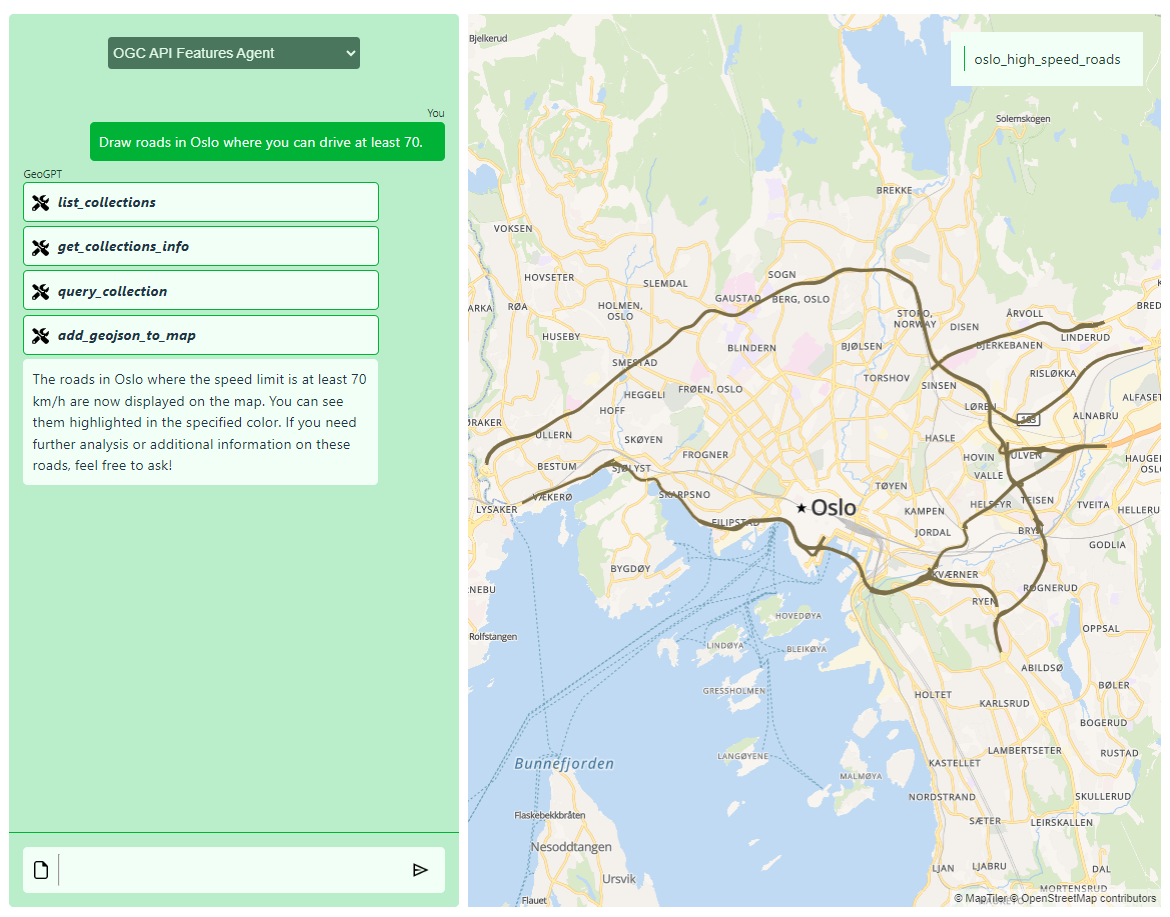
\includegraphics[width=\textwidth]{oslo_70kmh_oaf_novice.png}
        \caption{Novice-level prompting}
        \label{fig:novice-level-prompting-oslo-70kmh}
    \end{subfigure}
    \hfill
    \begin{subfigure}[b]{0.7\textwidth}
        \centering
        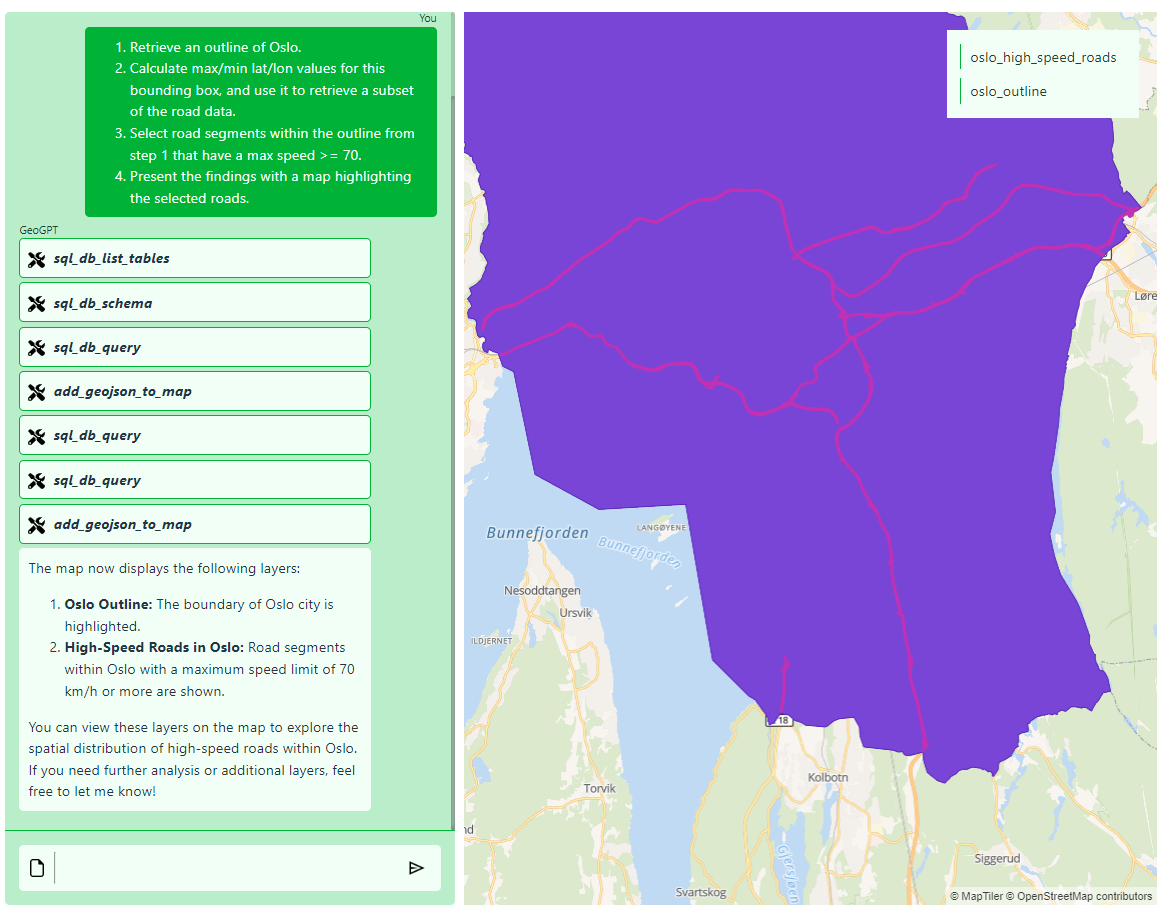
\includegraphics[width=\textwidth]{oslo_70kmh_sql_expert_sbs_2.png}
        \caption{Expert-level prompting}
        \label{fig:expert-level-prompting-oslo-70kmh}
    \end{subfigure}
    \caption{Comparison between novice- and expert-level prompting of \acrshort{acr:ogc} \acrshort{acr:api} Features agent for retrieval of high-speed roads in Oslo}
    \label{fig:novice-vs-expert-oslo-70kmh}
\end{figure}





\glsresetall

